\documentclass[a4paper]{article}
\usepackage[utf8]{inputenc}
\usepackage[russian]{babel}
\usepackage[T2]{fontenc}
\usepackage[warn]{mathtext}
\usepackage{graphicx}
\usepackage{amsmath}
\usepackage{floatflt}
\usepackage[left=20mm, top=20mm, right=20mm, bottom=20mm, footskip=10mm]{geometry}


\graphicspath{ {images/} }
\usepackage{multicol}
\setlength{\columnsep}{2cm}


\begin{document}

\begin{titlepage}
	\centering
	\vspace{5cm}
	{\scshape\LARGE Московский физико-технический институт \par}
	\vspace{4cm}
	{\scshape\Large Лабораторная работа \par}
	\vspace{1cm}
	{\huge\bfseries Эффект Холла в полупроводниках \par}
	\vspace{1cm}
	\vfill
\begin{flushright}
	{\large выполнила студентка 653 группы ФФКЭ}\par
	\vspace{0.3cm}
	{\LARGE Карпова Татьяна}
\end{flushright}
	

	\vfill

% Bottom of the page
	Долгопрудный, 2017 г.
\end{titlepage}

\section{Цель работы}
измерение подвижности и концентрации носителей заряда в полупроводниках

\section{В работе используются:}
\begin{itemize}
    \item электромагнит с источником питания
    \item амперметр
    \item миллиамперметр
    \item милливеберметр
    \item реостат
    \item источник питания (1,5 В)
    \item образцы легированного германия
\end{itemize}

\section{Теоретические положения}

\begin{floatingfigure}{41mm}
\noindent
\hfil
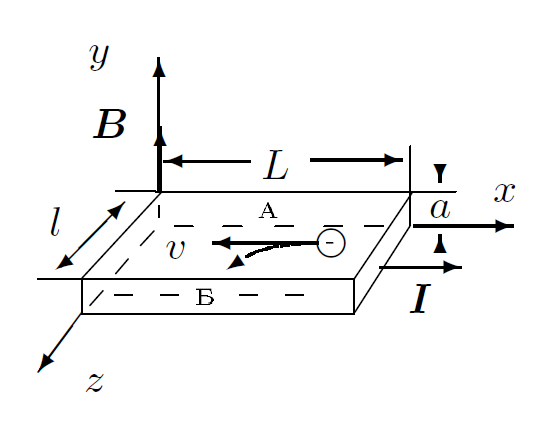
\includegraphics[width=41mm]{fig1.PNG}
\hfil
\caption{Образец с током в магнитном токе}
\label{figCurvesFF}
\end{floatingfigure}

На электрон, движущийся в магнитном поле, действует сила Лоренца. Также на пластине с током, помещённой в магнитное поле, возникает разность потенциалов. В итоге, сила, действующая на электрон:

\begin{equation}
    F_1 = -eE - e<v>B
\end{equation}


Под действием этой силы электроны отклоняются к грани Б, на грани А создаётся нескомпенсированный положительный заряд. Из-за разности потенциалов возникает электрическое поле, направленное от грани А к Б: $F_2 = eE_z$. Приравнивая $F_1$ и $F_2$, найдём ЭДС Холла:

\begin{equation}
    U_a_b = - \frac{IB}{nea} = -R_x \frac{IB}{a}
\end{equation}

Также в эксперименте проводится измерение удельной проводимости образца:

\begin{equation}
    \sigma = \frac{I L_3_4}{U_3_5 a l}
\end{equation}

\section{Экспериментальная установка}

\begin{figure}[h]
    \centering
    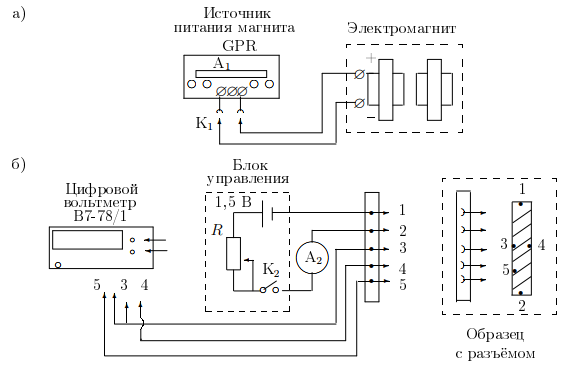
\includegraphics[width=10cm]{fig2.PNG}
    \caption{Схема установки для исследования эффекта Холла в полупроводниках}
    \label{fig:vac}
\end{figure}

\section{Выполнение работы}

\begin{enumerate}
    \item Проведём калибровку электромагнита - определим связь между индукцией магнитного поля в зазоре электромагнита и током через обмотку магнита. Для этого снимем зависимость магнитного потока Ф, пронизывающего катушку в поле, от тока $I_M$ ($\Phi = BSN$). Результаты занесём в таблицу 1, а также представим на графике. Уравнение для нахождения $B$ в зависимости от $I_M$: $B = -0.196I^2+0.91I$
    
    \begin{table}[h]
    \centering
    \begin{center}
    \caption{Калибровка электромагнита}
    \end{center}
    \vspace{0.1cm}
    \label{tab:my_label}
    \begin{tabular}{ |p{1.5cm}||p{0.7cm}|p{0.7cm}|p{0.7cm}|p{0.7cm}|p{0.7cm}|p{0.7cm}|p{0.7cm}|p{0.7cm}|  }
 \hline
$I_M, A$ & 0 & 0.3 & 0.6 & 0.9 & 1.2 & 1.5 & 1.8 & 2.08 \\
 \hline
 $\Phi, $мВб & 0.15 & 1.7 & 3.3 & 4.9 & 6.25 & 7.2 & 7.8 & 8.3\\
 \hline
 $B, $Тл & 0.021 & 0.236 & 0.458 & 0.681 & 0.868 & 1.000 & 1.083 & 1.153\\
 \hline
 
\end{tabular}
\end{table}
    
    \begin{figure}[h]
    \centering
    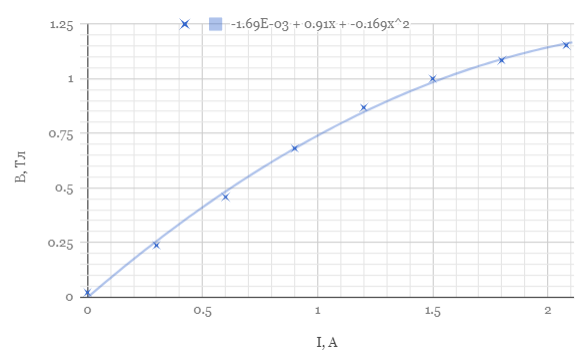
\includegraphics[width=15cm]{graph1.PNG}
    \caption{График калибровки электромагнита}
    \label{fig:vac}
\end{figure}
    
    \item Проведём измерение ЭДС Холла. Снимем зависимость напряжения $U_3_4$ от тока через обмотки магнита (с учётом $U_0$ при $I_M = 0$). Выполним серию экспериментов для различных токов через образец $I$ (от 0.3 до 1 мА). Результаты измерений занесём в таблицу 2, построим на одном графике семейство прямых $\Epsilon_X = f(B)$ (рис. 4)
    
    \begin{table}[h]
    \centering
    \begin{center}
    \caption{Зависимость напряжения в образце от тока в обмотке электромагнита}
    \end{center}
    \vspace{0.1cm}
    \label{tab:my_label}
    \begin{tabular}{ |p{3cm}||p{0.7cm}|p{0.7cm}|p{0.7cm}|p{0.7cm}|p{0.7cm}|p{0.7cm}|p{0.7cm}|p{0.7cm}|p{0.7cm}|p{0.7cm}|p{0.7cm}|  }
 \hline
$I_M, мA$ & 0 & 0.21 & 0.42 & 0.63 & 0.84 & 1.05 & 1.26 & 1.47 & 1.68 & 1.89 & 2.06\\
 \hline
 $B, $Тл & 0.000 & 0.184 & 0.352 & 0.506 & 0.645 & 0.769 & 0.878 & 0.973 & 1.052 & 1.116 & 1.157\\
 \hline
 \hline
$U_3_4, B (I = 0.3$мА) & 0.069 & 0.088 & 0.107 & 0.126 & 0.142 & 0.156 & 0.169 & 0.177 & 0.184 & 0.189 & 0.192\\
\hline
$U_3_4, B (I = 0.4$мА) & 0.092 & 0.116 & 0.143 & 0.167 & 0.189 & 0.208 & 0.225 & 0.236 & 0.245 & 0.251 & 0.255\\
\hline
$U_3_4, B (I = 0.5$мА) & 0.115 & 0.146 & 0.178 & 0.209 & 0.237 & 0.26 & 0.281 & 0.295 & 0.305 & 0.301 & 0.319\\
\hline
$U_3_4, B (I = 0.6$мА) & 0.139 & 0.175 & 0.215 & 0.254 & 0.285 & 0.313 & 0.338 & 0.356 & 0.368 & 0.378 & 0.383\\
\hline
$U_3_4, B (I = 0.7$мА) & 0.161 & 0.205 & 0.25 & 0.293 & 0.332 & 0.366 & 0.394 & 0.415 & 0.429 & 0.441  &  \\
\hline
$U_3_4, B (I = 0.8$мА) & 0.184 & 0.233 & 0.286 & 0.335 & 0.38 & 0.416 & 0.449 & 0.473 & 0.483 & 0.502 & 0.509\\
\hline
$U_3_4, B (I = 1.0$мА) & 0.231 & 0.292 & 0.358 & 0.418 & 0.457 & 0.521 & 0.563 & 0.591 & 0.613 & 0.629 & 0.635\\
\hline
\hline

 \end{tabular}
\end{table}

\begin{figure}[h]
    \centering
    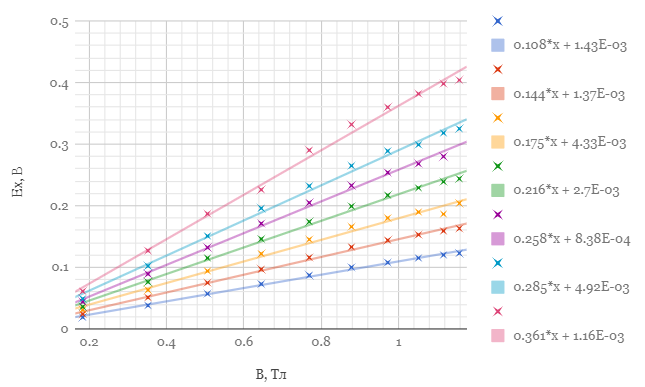
\includegraphics[width=\textwidth]{graph2.PNG}
    \caption{Семейство зависимостей ЭДС Холла от магнитного воля в электромагните при разных токах через образец}
    \label{fig:vac}
\end{figure}
\par

\begin{figure}[h]
    \centering
    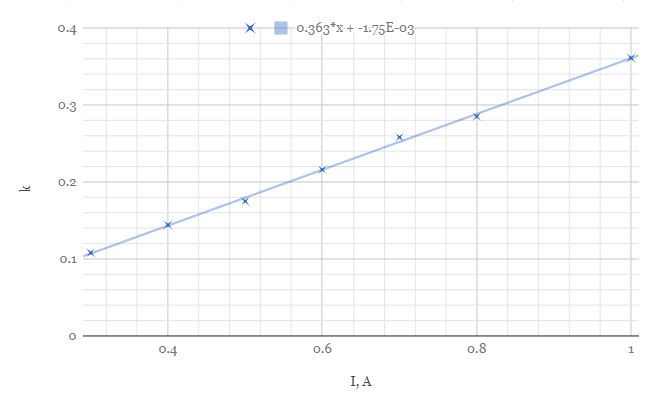
\includegraphics[width=15cm]{graph3.PNG}
    \caption{Определение постоянной Холла}
    \label{fig:vac}
\end{figure}

\item Определив угловые коэффициенты прямых рис.4, построим график зависимости $K = f(I)$ (рис. 5). По этому графику определим величину постоянной Холла. Погрешность рассчитаем по методу наименьших квадратов, учитывая погрешности приборов



\begin{center}
  $R_x = - k a = 0.363 * 2.2 = (7.98 \pm 0.69)10^-^4 $ м$^3$/Кл  
\end{center}

Относительная погрешность составляет 8,6\%.

\item Учитывая рис. 1, направление тока в образце и знак ЭДС Холла, определим характер проводимости в образце по правилу векторного произведения. Проводимость электронная.

\item Рассчитаем концентрацию носителей тока:

\begin{center}
    $n = \frac{1}{R_x e} = (0.78 \pm 0.21)$ед/м$^3$
\end{center}

По формуле (3) рассчитаем удельную проводимость исследуемого образца. При $I = 1$ мА $U_3_5 = 2.16 $В, параметры установки: $a = 2.2mm, l = 7 mm, L_3_5 = 6 mm$
 \begin{center}
     $\sigma = 148.9$ 1/(Ом м)
 \end{center}
 
 Наконец, рассчитаем подвижность носителей в образце.
 \begin{center}
     $b = \frac{\sigma}{ne} = 1448 \pm 350 $см$^2$/(В*с) \\
     $b_{theor} = 3800$ см$^2$/(В*с) для электронной проводимости
 \end{center}
\end{enumerate}

\section{Вывод}

В ходе работы был исследован эффект Холла в полупроводнике-германии. Были определены такие характеристики, как постоянная Холла, концентрация холловских частиц, удельная электрическая проводимость германия и подвижность электронов-носителей заряда в нём. Результаты совпали с табличными по порядку величины. Возможная причина несовпадения - характер проводимости в исследуемом образце не чисто электронный, а электронно-дырочный (подвижность носителей заряда уменьшится). \\
Был проведён небольшой опрос среди студентов, выполнявших эту работу. Выяснилось, что на одной установке (у окна) полученное значение подвижности электронов сходилось с табличным, а на другой (ближе к двери) - была меньше практически на 2000 единиц. Самое разумное объяснение этого - то, что исследуемый образец не является чистым германием, а лигированным, с иными свойствами. Даже мельчайшие доли примесей способны изменять подвижность носителей заряда на тысячи единиц.


\end{document}
